%\documentclass[a4paper,12pt,oneside,pdflatex,italian,final,twocolumn]{article}
\documentclass[a4paper,12pt,oneside,pdflatex,italian,final]{article}

\usepackage[utf8]{inputenc}
\usepackage{parallel}
\usepackage{siunitx}
\usepackage{booktabs}
\usepackage{fancyhdr}
\usepackage{subcaption}
\usepackage{minted}
\usepackage{hyperref}
\usepackage{pdfpages}

\usepackage[export]{adjustbox}
\usepackage[margin=0.5in]{geometry}
\addtolength{\topmargin}{0in}

\usepackage{libertine}
\renewcommand*\familydefault{\sfdefault}  %% Only if the base font of the document is to be sans serif
\usepackage[T1]{fontenc}

\hypersetup{
	colorlinks=true, %set true if you want colored links
	linktoc=all,     %set to all if you want both sections and subsections linked
	linkcolor=blue,  %choose some color if you want links to stand out
	urlcolor=blue,   %url color
}

\definecolor{LightGray}{gray}{0.95}

\title{Logic Motor Driver}
\author{Achmadi ST MT}
\date{July 2024}

\begin{document}
	\pagestyle{fancy}

	\lhead{Achmadi}
	\chead{\today}
	\rhead{Summary Document}

	\section{Schematic Design}

    \begin{figure}[h]
        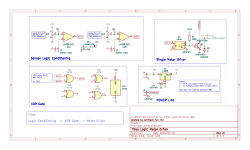
\includegraphics[width=\textwidth]{images/logic_driver.png}
    \end{figure}
    
    \section{Design Motes}
    
    Some notes for each schematic blocks:
    \begin{itemize}
    	\item Sensor Input Conditioning:
    	\begin{itemize}
    		\item Using Comparator to create logic signal with 0.6v as logic barrier.
    		\item Currently using potensiometer as reference voltage for comparator op-amp
    		\item Should be use better reference voltage but still not found myself
    		\item Using GND as VSS might not work
    	\end{itemize}
    	
    	\item XOR Logic
    	\begin{itemize}
    		\item Using 7040 series chip as XOR gate
    		\item Logic voltage level is 5V as VCC/VDD both for comparator and XOR gate is 5V
    	\end{itemize}
    	
    	\item Motor Driver
    	\begin{itemize}
    		\item Using 4n35 as low voltage signal isolation
    		\item IRG45PF not as good as IGBT series, but run in VCE 15V for control more than 200V drive
    		\item Small diode to prevent induction back voltage
    	\end{itemize}
    	
    	\item Power Line
    	\begin{itemize}
    		\item Using 7805 to get 5V from 15V
    		\item Separated GND and GNDPWR (for 100V) using Schottky diode 
    	\end{itemize}
    \end{itemize}
    
    \newpage
    \section{PCB Draft}
    
    \begin{figure}[h]
    	\includegraphics[width=\textwidth]{images/logic_driver_pcb.png}
    \end{figure}
    
    Notes: 2mm Wire for motor line should be enough
    
    \begin{figure}[h]
    	\includegraphics[width=\textwidth]{images/logic_driver_3d.png}
    \end{figure}
    
    
    \section{Repository}
    
    The KiCAD (on version 7) design above can be found on my Github here:
    
    \url{https://github.com/mekatronik-achmadi/short-jobs/tree/master/recruitmen/formulatrix/logic_driver}
    
\end{document}
